\documentclass[oneside,final,14pt]{extarticle} %размер бумаги устанавливаем А4, шрифт 12пунктов
\usepackage[utf8]{inputenc}
\usepackage[T2A]{fontenc}
\usepackage[english,russian]{babel}%используем русский и английский языки с переносами
\usepackage{indentfirst}
\setlength{\parindent}{1.25cm}
\linespread{1.5}
\usepackage{pdfpages}
\sloppy
\usepackage{graphicx} %хотим вставлять в диплом рисунки?
\graphicspath{ {../img/} } %теперь все пути рисунков отсчитываются от папки img
\usepackage{amssymb,amsfonts,amsmath,mathtext,cite,enumerate,float} %подключаем нужные пакеты расширений
\usepackage{titlesec} %хотим вставлять в диплом рисунки?



\titleformat{\section}{\filcenter\normalfont\Large\bfseries}{\thesection.}{0.6em}{}
\titleformat{\subsection}{\filright\normalfont\large\bfseries}{\thesubsection.}{0.4em}{}

\usepackage{lipsum,mathptmx,etoolbox}

\makeatletter
\patchcmd{\@makechapterhead}{\huge}{\large}{\bfseries}{}
\patchcmd{\@makechapterhead}{\Huge}{\large}{\bfseries}{}
\patchcmd{\@makeschapterhead}{\Huge}{\large}{\bfseries}{}
\makeatother

\usepackage{geometry} % Меняем поля страницы
\geometry{left=3cm}% левое поле
\geometry{right=1cm}% правое поле
\geometry{top=2cm}% верхнее поле
\geometry{bottom=2cm}% нижнее поле



\pagestyle{plain}

\begin{document}


\includepdf[offset=0cm -0cm]{titulny_list_bak.pdf}

\setcounter{page}{2}

\setlength{\parindent}{1.25cm}

\tableofcontents
\newpage

\section*{Введение}
\addcontentsline{toc}{section}{Введение}
ЕГЭ (Единый государственный экзамен) – это государственный экзамен, проводимый в России для выпускников школ. ЕГЭ проводится по 14 предметам, включая французский, испанский, немецкий и с 2019 года китайский язык. Обязательными являются русский язык и базовый или профильный модуль по математике.

ЕГЭ проходит каждый год в период с мая по июль. Цель экзамена – определить уровень знаний и умений выпускников и принять решение о поступлении в высшие учебные заведения. Результаты ЕГЭ засчитываются как вступительное испытание в вузы России. Сдают ЕГЭ выпускники средних школ, которые получили документ об окончании общеобразовательной школы. В целом, это молодые люди в возрасте 16-18 лет.

Для успешной сдачи ЕГЭ необходима тщательная подготовка, и немаловажную роль в этом играет сайт «Решу ЕГЭ»[4]. Он может быть полезен в подготовке к экзамену по математике. Однако за время подготовки к экзаменам школьники быстро сталкиваются с дефицитом заданий, а в некоторых случаях прибегают к списыванию.

«Час ЕГЭ» — компьютерный образовательный проект, разрабатываемый при математическом факультете ВГУ в рамках «OpenSource кластера» и предназначенный для помощи учащимся старших классов подготовиться к тестовой части единого государственного экзамена.

Задания в «Час ЕГЭ» генерируются случайным образом по специализированным алгоритмам, называемых шаблонами, каждый из которых охватывает множество вариантов соответствующей ему задачи. В настоящее время в проекте полностью реализованы тесты по математике с кратким ответом. Планируется с течением времени включить в проект тесты по другим предметам школьной программы. 

Цель - разработка шаблонов, основанных на задачах из ЕГЭ [5]. Большое и разнообразное количество заданий, генерируемых алгоритмами шаблонов, позволяет объективно оценить знания школьников. Благодаря им решаются проблемы списывания и нехватки заданий.
\newpage

\section{Виртуальные машины VirtualBox}
\subsection{Установка VirtualBox и Ubuntu}

\begin{figure}
\quad 1.\quad Перейходим по ссылке https://www.virtualbox.org. Нажимаем кнопку “Download”, выбираем «Windows hosts» и устанавливаем «VirtualBox».

		\centering
		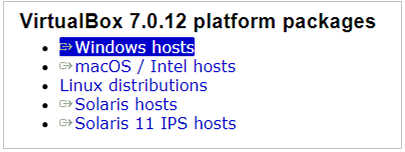
\includegraphics[width=0.65\linewidth]{img/1.png}
\caption{«Windows hosts».}
\label{ris:image}
\end{figure}

\begin{figure}
\quad 2.\quad Далее, для того чтобы любая виртуальная машина могла работать, необходимо включить виртуализацию. Чтобы проверить, включена ли она у вас, откройте диспетчер задач и перейдите в раздел «Производительность». Откройте окно диспетчера задач на весь экран и внизу вы увидите, включена ли виртуализация.

		\centering
		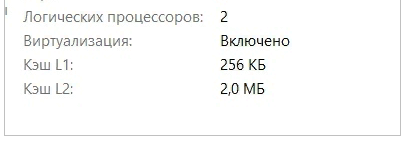
\includegraphics[width=0.65\linewidth]{img/2.png}
\caption{Диспетчер задач. Виртуализация.}
\label{ris:image}
\end{figure}

\begin{figure}
\quad Если виртуализация у вас выключена, то вам необходимо войти в BIOS. Для этого нужно нажать на кнопку «Перезагрузить компьютер», и, как только он начинает запускаться, зажать клавишу «Esc» ( или начать нажимать много раз на клавишу delete, пока не запустится «Startup menu». Зависит от того, ноутбук у вас или компьютер), после чего и откроется «Startup menu». Чтобы открыть BIOS нажмите клавишу «F10». Перейдите в «System Configuration» нажав два раза на кнопку со стрелочкой вправо. Затем спуститесь до «Virtualization Technology», нажав на кнопку со стрелочкой вниз и нажмите клавишу «Enter». Выберите «Enable» и снова нажмите «Enter». Нажмите клавишу «F10» и выберите «Yes». После чего компьютер перезагрузится уже с включённой виртуализацией.

		\centering
		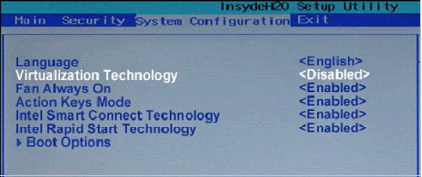
\includegraphics[width=0.65\linewidth]{img/3.png}
\caption{BIOS. «Virtualization Technology».}
\label{ris:image}
\end{figure}

\begin{figure}
3. Скачиваем «Ubuntu» с официального сайта по ссылке: https://ubuntu.com/download/desktop. Затем открываем «VirtualBox» и нажимаем кнопку «Создать». Заполняя все поля, необходимо указать объём памяти не менее 2 гигабайт, иначе «Ubuntu» просто не запустится. В остальном можно принять все установки по умолчанию. После создания, необходимо нажать на кнопку «Настройки», далее «Носители», у надписи «Контроллер: IDE» нажать на значок диска с плюсиком.

		\centering
		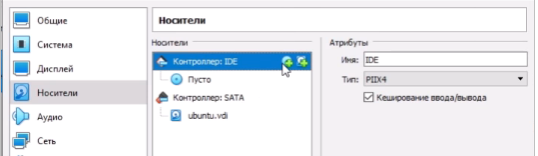
\includegraphics[width=0.65\linewidth]{img/4.png}
\caption{Настройки. Носители.}
\label{ris:image}

\end{figure}

\begin{figure}
\quad Затем «Добавить» и выбрать скаченный ранее файл с «Ubuntu». После чего можно нажать кнопку «Запустить». После запуска, мы выбираем язык, нажимаем скачать «Ubuntu», заполняем все поля, и выбираем параметры по умолчанию. И наконец видим интерфейс «Linux».
\end{figure}



\newpage

\subsection{Снимки виртуальной машины}
Обновлением виртуальной машины, или неудачная попытка настройки или просто какая-то ошибка при её запуске, может привести к потери ценных данных, а на переустановку системы и настройку программ может уйти очень много времени. Именно для таких случаев и предназначены снимки в VirtualBox. Они нужны для сохранения прогресса на случай, непредвиденной поломки машины, и отката до ранее стабильного состояния. Поэтому перед и после обновления или установки чего-то важного, стоит делать снимки.

Для создания снимка своей виртуальной машины нужно нажавть на кнопку с изображением фотоаппарата с плюсом.

Снимок можно удалить, восстановить и посмотреть на его свойства на момент его создания.

\begin{figure}[h]
		\centering
		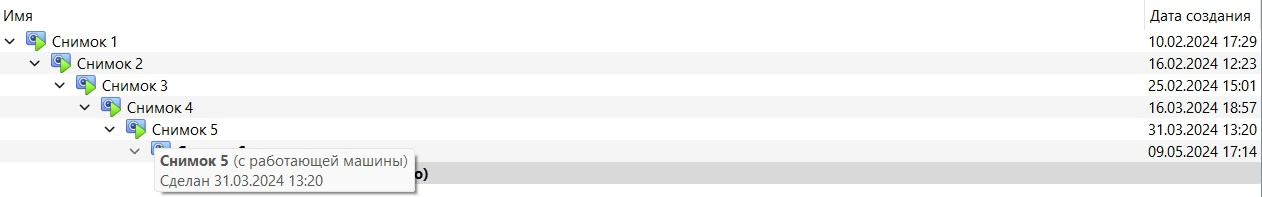
\includegraphics[width=1\linewidth]{VM/s2.jpg}
\caption{Дерево снимков.}
\label{ris:image}
\end{figure}

При создании можно оставить название по умолчанию и не вводить никакого описания, но если таких снимков в будущем накопится много, можно будет запутаться. 

\begin{figure}[h]
		\centering
		
\includegraphics[width=0.8\linewidth]{VM/s3.jpg}
\caption{Действия со снимками.}
\label{ris:image}
\end{figure}

Для восстановления состояния виртуальной машины нужно выбрать нужный нам снимок, и нажать «Восстановить снимок».
 
VirtualBox предложит дополнительно создать снимок текущего состояния системы. Нужно поставить галочку и нажать кнопку «Восстановить». чтобы, иметь возможность вернуться к  текущему состоянию, если была совершена ошибка или снимок оказался не тот, что нужен.
 
\begin{figure}[h]
		\centering
		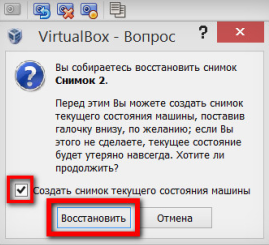
\includegraphics[width=0.4\linewidth]{VM/s4.png}
\caption{Восстановление снимка.}
\label{ris:image}
\end{figure}

Далее можно дать снимку текущего состояния имя и описание и нажать кнопку «ОК».

После VirtualBox вернёт состояние системы к моменту создания выбранного снимка.


\newpage

\subsection{Клонирование виртуальной машины}
\quad 1.\quad В ходе работы с виртуальной машиной возникла необходимость перенести её с одного своего устройства на другое.
\newline Для этого открываем Virtual Box, нажимаем правой кнопкой мыши по своей виртуальной машине и выбираем пункт клонировать. В появившемся окне указываем имя нового клона и его путь по которому он будет сохранён. Так же в графе «Политика MAC-адреса» выбираем вариант: «Сгенерировать новые MAC-адреса всех сетевых адаптеров».

\begin{figure}[h]		
		\centering
		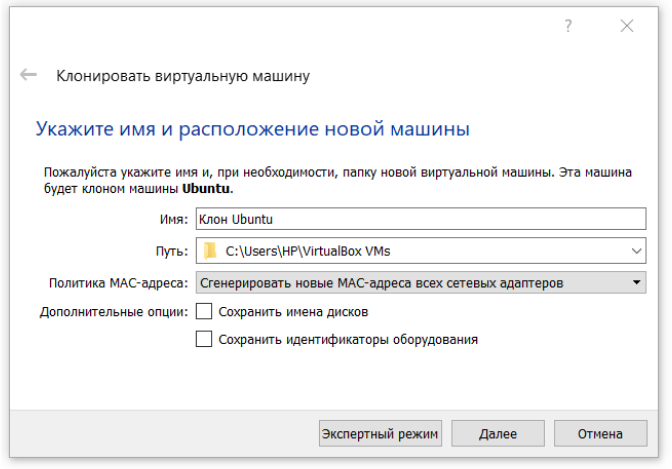
\includegraphics[width=0.6\linewidth]{VM/8.png}
\caption{Окно клонирования.}
\label{ris:image}
\end{figure}

\quad В следующем окне нужно было указать тип клонирования: полное или связное. При связном клонировании будет создана новая машина, использующая файлы виртуальных жёстких дисков клонируемой машины и нельзя перенести её на другой компьютер без переноса клонируемой. При полном клонировании, будет создана полная копия клонируемой виртуальной машины (включая все файлы виртуальных жёстких дисков). Поэтому выбиираем полное клонирование.

\quad В окне с указанием цели клонирования, указываем клонировать всё, чтобы новая машина не только отражала текущее состояние клонируемой машины, но и имела копии всех снимков её древа снимков.

\quad Далее нажимаем на кнопку «клонировать», после чего запускается процесс клонирования. По его завершению переносим новую машину на флэшку. Это можно сделать нажав в Virtual Box на клон правой кнопкой мыши и выбрать пункт «Переместить». Или просто зайти в папку, в которую был сохранён наш клон, и переместить его уже оттуда.

\quad Далее подсоединяем флэшку к другому компьютеру и переносим машину в папку Virtual Box. Открыв Virtual Box, нажиимаем вверху на кнопку «Машина» и выбрал пункт добавить. После чего находим свою машину и нажал кнопку «Открыть».

\begin{figure}[h]
		\centering
		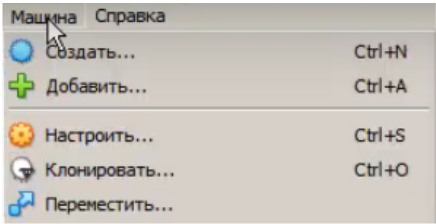
\includegraphics[width=0.4\linewidth]{VM/9.png}
\caption{Добавление виртуальной машины.}
\label{ris:image}
\end{figure}

\quad Виртуальная машина добавлена. Но зайдя в настройки, можно увидеть, что объём выделенной основной памяти составляет всего лишь 2 гигабайта, что слишком мало для работы с машиной. Так как наша машина находится в состоянии «Сохранена», мы не можем изменять её настройки. Поэтому нажимаем правой кнопкой мыши по перенесённому клону, и выбираем пункт «Сбросить сохранённое состояние». После чего снова нажимаем правой кнопкой мыши по машине, выбираем пункт «Настроить…» и в «Системе» выделяем нужное количество памяти.

\begin{figure}[h]
		\centering
		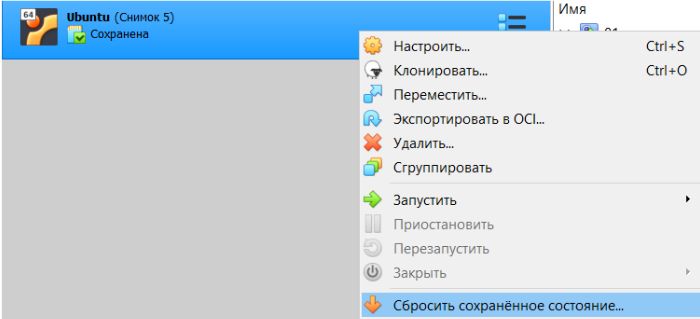
\includegraphics[width=0.75\linewidth]{VM/10.png}
\caption{Настройка памяти.}
\label{ris:image}
\end{figure}

\quad Далее заходим в «Носители» и выбираем свой жёсткий диск, так как иначе при запуске виртуальной машины мы бы ничего не увидели.

\begin{figure}[h]
		\centering
		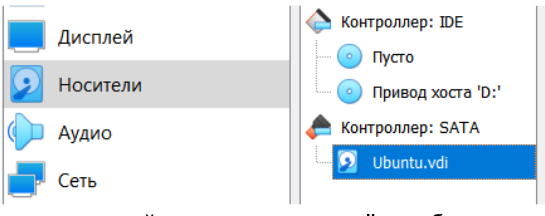
\includegraphics[width=0.5\linewidth]{VM/11.png}
\caption{Настройки. Носители.}
\label{ris:image}
\end{figure}

\quad Теперь клон виртуальной машины перемещён, добавлен на новый компьютер и с ним можно работать.

\quad Есть и альтернативный способ переноса виртуальной машины с одного устройства на другое, с помощью функций «Экспорт» и «Импорт».

\begin{figure}[h]
\centering Экспорт виртуальной машины
\label{ris:image}
\end{figure}

\quad Экспорт конфигурации виртуальной машины происходит в файл формата .ova (Open Virtual Appliance). Это универсальный формат для хранения данных виртуальной машины, файлы .ova могут использоваться в разных программах виртуализации: VirtualBox, VMware Workstation, Microsoft Hyper-V. Виртуальная машина, экспортированная в файл .ova, затем может быть импортирована как в VirtualBox, так и в VMware Workstation, Microsoft Hyper-V.

\quad В меню программы нужно зайти в «Файл» и выбрать пункт «Экспорт конфигураций». В открывшемся окне выбираем машину для экспорта, и нажимаем «Далее».

\begin{figure}[h]
		\centering
		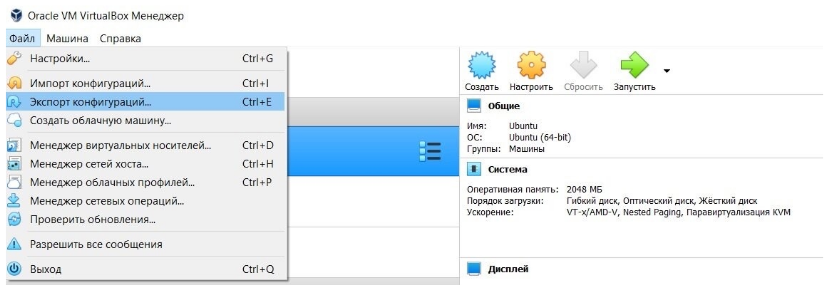
\includegraphics[width=0.8\linewidth]{VM/12.png}
\caption{«Экспорт конфигураций».}
\label{ris:image}

\end{figure}

\quad Выбираем место размещения после экспорта. Также лучше выбрать «Включать МАС-адреса всех сетевых адаптеров», нажимаем «Далее». 

\begin{figure}[h]
		\centering
		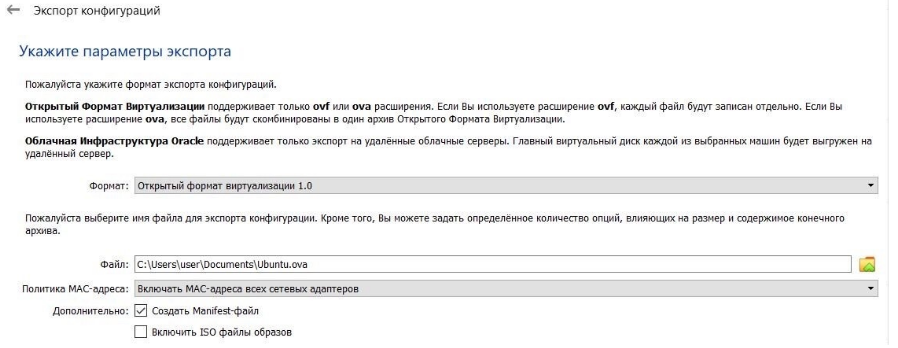
\includegraphics[width=1\linewidth]{VM/13.png}
\caption{МАС-адреса сетевых адаптеров.}
\label{ris:image}
\end{figure}

\quad В следующем окне оставляем всё без изменений, и нажимаем кнопку “Экспорт”. Сам экспорт может занимать несколько минут, в зависимости от размера виртуальной машины. После экспорта в указанном месте создается файл, который уже необходимо будет импортировать.

\begin{figure}[h]
\centering Импорт виртуальной машины
\label{ris:image}
\end{figure}

\quad Теперь необходимо скопировать файл на флэшку. Или же можно воспользоваться облочным хранилищем, так как возможно при попытке перенести его на флешку, может возникнуть ошибка: «Файл слишком велик для конечной файловой системы». Она возникает, если передаётся файл размером более четырёх гигабайт на носитель, неспособный с ним работать. Для устранения этой ошибки можно воспользоваться форматированием флешки или разбитием файла с виртуальной машины на несколько частей. Был также опробован способ сжатия виртуальной машины в zip файл, но она оказалась практически без сжимающий составляющих.

\quad Далее на втором компьютере заходим в программу Virtual Box и нажимаем вверху «Файл» и выбираем пункт «Импорт конфигураций».

\begin{figure}[h]
		\centering
		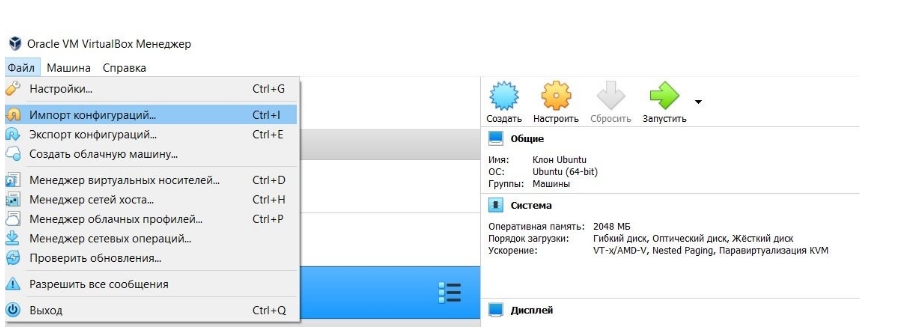
\includegraphics[width=1\linewidth]{VM/14.png}
\caption{Импорт конфигураций.}
\label{ris:image}
\end{figure}

\quad В окне импорта выбираем место размещения файла виртуальной машины, нажимаем «Далее». В следующем окне можно изменить параметры импорта, например, увеличить количество процессоров. Также желательно «Включать (сгенерировать новые) МАС-адреса всех сетевых адаптеров», и нажимаем «Импорт».

\quad Импорт также как и экспорт в зависимости от размера виртуальной машины может занимать несколько минут.

\quad После импорта виртуальная машина появляется в списке и с ней уже можно будет работать.
\newpage

\subsection{Увеличение объёма памяти виртуальной машин}
\begin{figure}
\quad В какой-то момент при работе за виртуальной машиной, высветилось сообщение о том, что память заканчивается. 
\end{figure}

\begin{figure}
\quad Для начала вводим в поисковике Linux-а «Диск» и, нажав на иконку диска, смотрим насколько он заполнен, и сколько памяти осталось. 
\end{figure}

\begin{figure}
\quad Необходимо выключить виртуальную машину, а не сохранить, чтобы можно было изменить её настройки. Далее в меню VirtualBox выбираем пункт «Файл» и нажимаем на «Менеджер виртуальных носителей…».
\end{figure}

\begin{figure}
\quad В открывшемся окне заходим в свойства диска и находим его размер. Двигая за ползунок, изменяем его объём с 16 гигабайт до 30 и нажимаем «Применить». 
\end{figure}

\begin{figure}
\quad При повторном открытии виртуальной машины было обнаружено, что размер памяти не изменился. Мы пришли к выводу, что для того чтобы увеличить объём памяти жёсткого диска, нужно сделать клон текущего состояния виртуальной машины или удалить снимки. К сожалению изменять размер диска, просто нельзя, пока существуют его точки сохранения. Поэтому снова выключаем машину, и делаем клон её текущего состояния. Он делается точно так же, как когда мы делали клон для переноса его с одного устройства на другое. Единственное отличие в том, что в этот раз выбираем клонировать не всё, а только текущее состояние. 
\end{figure}

\begin{figure}
\quad Увеличив в «Менеджере виртуальных носителей…» уже объём памяти клона, заходим в настройки виртуальной машины, увеличиваем размер памяти в «Системе» и выбраем соответствующий диск в «Носителях», так же как это делали, после переноса клона на другое устройство. Далее запускаем новую машину и заходим в «Диск», где виидим, что его размер стал больше, и появилась дополнительная область памяти.
\end{figure}

\begin{figure}
\quad Чтобы задействовать его, нажиимае на иконку настроек, сдвигаем ползунок до конца вправо, чтобы можно было использовать всю новую память и нажиимаем «Применить», после чего вводим свой пароль. Но опять ничего не получилось. Чтобы наконец всё заработало, нужен установочный файл Ubuntu нашей виртуальной машины. Он остался на прошлом устройстве, с которого мы и клонировали машину. Воспользовавшись гугл диском, перенесли файл, так как флэшка не позволяет загрузить в неё что-либо весом более 4 гигабайт без её форматирования.
\end{figure}
\newpage

\section{Работа с GitHub}
\subsection{Установка git, nodejs, npm и grunt}
Для установки всего необходимого, нам нужно открыть терминал, нажав на его иконку. 

\begin{figure}[h]
		\centering
		
\includegraphics[width=0.2\linewidth]{VM/5.png}
\caption{Терминал.}
\label{ris:image}
\end{figure}

Далее, для скачивания, необходимо ввести соответствующие строки кода:
\newline \texttt{git – sudo apt install git}
\newline \texttt{nodejs – sudo apt install nodejs}
\newline \texttt{npm - sudo apt install npm}
\newline \texttt{grunt - sudo apt install grunt}
\newline Чтобы удостовериться, что всё правильно скачалось, можно узнать версию данного продукта. Например: \texttt{git –version}
\newpage

\subsection{Работа с репозиторием}
Для работы с репозиторием сначала нужно зарегестрироваться на GitHub, перейдя по ссылке: : https://github.com/ и заполнить всю необходимую информацию о себе.

Затем переходим по ссылке: https://github.com/nickkolok/chas-ege/. Далее нажимаем на зелёную кнопку с надписью «Code», и копируем ссылку репозитория. Лучше сделать это сразу, потому что Ubuntu на VirtualBox может сильно нагружать компьютер, и открыть вкладку с браузером может быть проблематично из-за нагрузки. (Если возникли проблемы с копирование ссылки, то можно открыть браузер внутри Ubuntu, перейти по ссылке и скопировать ссылку репозитория в нём.)

\begin{figure}[h]
		\centering
		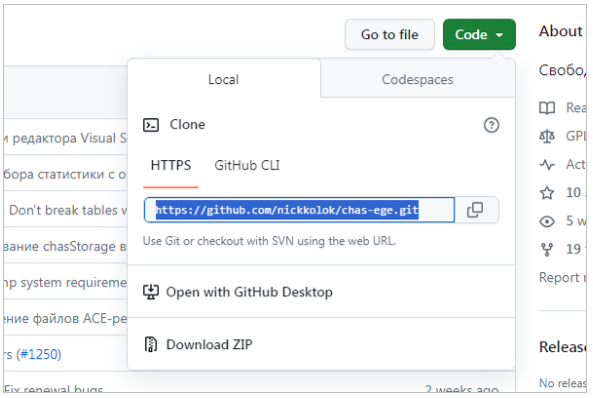
\includegraphics[width=0.9\linewidth]{VM/6.png}
\caption{Github. Ссылка на репозиторий.}
\label{ris:image}
\end{figure}

• Далее снова заходим в терминал и создаём папку на рабочем столе командой: mkdir <название папки>. Можно убедиться, что папка создана, с помощью команды: ls. Мы увидим все папки на рабочем столе, среди которых должна быть только что созданная.Затем заходим в папку командой: cd <название папки>, и клонируем себе репозиторий командой: git clone <ссылка на репозиторий >

• Добавляем себе ссылку на основной репозиторий проекта с помощью команды: git remote add upstream <ссылка на репозиторий> и убеждаемся, что он подключился, командой: git fetch upstream 

• Собираем проект командой: grunt. Важно выполнять эту команду в папке, в которую мы и склонировали репозиторий.

• Открываем файл dist/sh/otladka.html в браузере командой: «open otladka.html», и запускаем любой шаблон, для проверки, в открывшемся окне.


\begin{figure}[h]
		\centering
		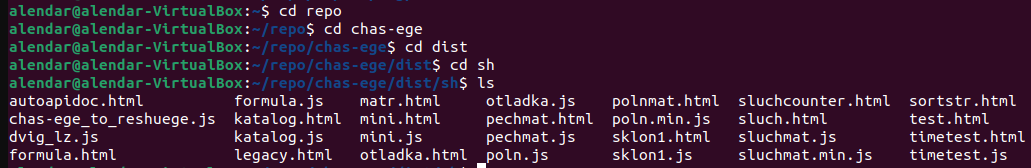
\includegraphics[width=1\linewidth]{VM/7.png}
\caption{Путь к файлу otladka.html.}
\label{ris:image}
\end{figure}
\newpage

\subsection{Создание SSH ключа}
Создание SSH ключа для возможности подключиться к удалённому репозиторию происходит в несколько этапов.
Для начала нужно проверить наличие ключа, введя следующие команды:
\newline \texttt{cd ~/.ssh}
\newline \texttt{ls}

Если файлов с названиями \texttt{id\_dsa} и \texttt{id\_dsa.pub} нет (открытый и приватный ключ), то можно создать их используя команду:
\newline  \texttt{ssh-keygen -o}
\newline \quad Далее нужно открыть содержимое файла dsa.pub командой:
\newline  \texttt{cat ~/.ssh/ id\_dsa.pub}

Далее добавили свой ключ себе в аккаунт на GitHub, чтобы иметь возможность подключиться к удалённому репозиторию [2]. А также прописали ещё одну команду, необходимую для подключения.

\begin{figure}[h]
		\centering
		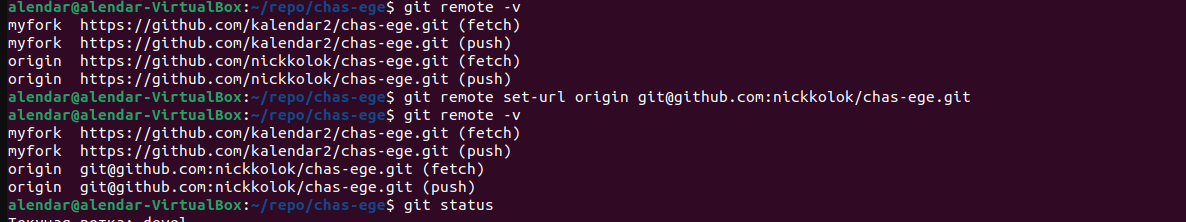
\includegraphics[width=1\linewidth]{VM/pod.png}
\caption{Подключению к удалённому репозиторию с помощью команды.}
\label{ris:image}
\end{figure}

Перейдя в репозиторий на GitHub «ЧАС-ЕГЭ», нужно нажать кнопку «Fork» справа вверху.

Открыв VirtualBox и войдя в свою виртуальную машину, открыли терминал и перешли в папку с «Час ЕГЭ» с помошью команды cd git/chas-ege.

Представление гиту выглядит следующим образом:
\newline \texttt{git config --global user.name «Фамилия Имя»}
\newline \texttt{git config --global user.email «электронная почта пользователя»}
\newline Можно придать выводу гита красные и зелёные цвета с помощью команд:
\texttt{git config --global color.ui true}
\newline Добавление своего форка на гитхаб в список удалённых репозиториев:
\texttt{git remote add myfork git@ github.com:«GitHubNik»/chas-ege.git}, где «GitHubNik» - ник пользователя на гитхабе. 

Основные команды для создания и отправления изменений в удалённый репозиторий:
\\Переключение на основную ветку (devel):
\\ \texttt{git checkout devel}
\\ \quad Её обновление (В некоторых случаях применима также команда: \texttt{git pull origin devel}):
\\ \texttt{git fetch origin devel}
\\ \quad Создание новой ветки:
\\ \texttt{git checkout -b newtask-777}
\\ \quad Проверка изменений, а также самой ветки:
\\ \texttt{git status}
\\ \quad Добавление всех изменений:
\\ \texttt{git add .}
\\ \quad Добавление всех изменений:
\\ \texttt{git commit -m «Внесены изменения в файл ...»}
\\ \quad Отправка изменений в удалённый репозиторий:
\\ \texttt{git push myfork newtask-777:myfork newtask-777:}
\newpage

\subsection{Игнорирование файлов}
Для того, чтобы сообщить Git, какие ненужные файлы или каталоги нужно игнорировать, можно создать .gitignore файл.

Для этого необходимо открыть Терминал и перейти к расположению репозитория Git. Далее создаётся файл для репозитория, с помощью команды \texttt{touch .gitignore}.

Если файл уже был отправлен в репозиторий, необходимо отменить отслеживание файла, прежде чем добавлено правило игнорирования, с помощью команды: \texttt{git rm --cached FILENAME}.

Файл невидим, как и все файлы с точкой в начале названия файла, но его можно увидеть с помощью команды \texttt{ls -a}. Зайдя в него, нужно записать путь к файлу или каталогу, который будет игнорироваться.

\begin{figure}[h]
		\centering
		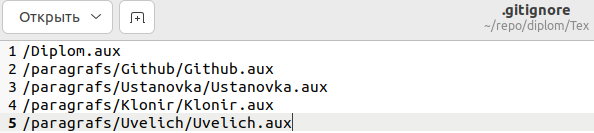
\includegraphics[width=0.6\linewidth]{VM/gitignore.png}
\caption{Файл .gitignore с списком файлов для игнорирования в нём.}
\label{ris:image}
\end{figure}

Это не единственный способ задания игнорирования файла или каталога. Можно также сообщить Git всегда игнорировать определенные файлы во всех репозиториях на компьютере. Для этого, например, каталог нужно добавить в файл с именем ignore , расположенным внутри каталога \texttt{~/.config/git}.

Также можно вообще не создавать файл .gitignore. Этот метод можно использовать для локально создаваемых файлов, которые не должны создавать другие пользователи. Для этого, используя текстовый редактор, нужно открыть файл, вызываемый \texttt{.git/info/exclude} в корневом каталоге репозитория Git.
\newpage

\section{Практическая реализация шаблонов}
\subsection{Примеры задач и их код}
\textbf{Пример пары заданий одного типа, на основе которых создан следующий шаблон. } 

\begin{figure}[h]
		\centering
		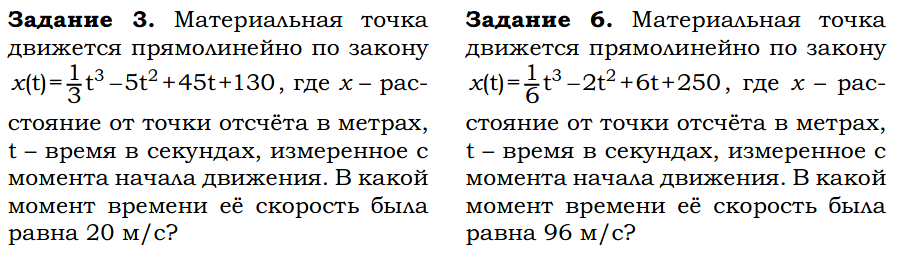
\includegraphics[width=1\linewidth]{VM/Пример.png}
\label{ris:image}
\end{figure}

Первая часть шаблона выглядит следующим образом:

	\begin{figure}[h]
		\centering
		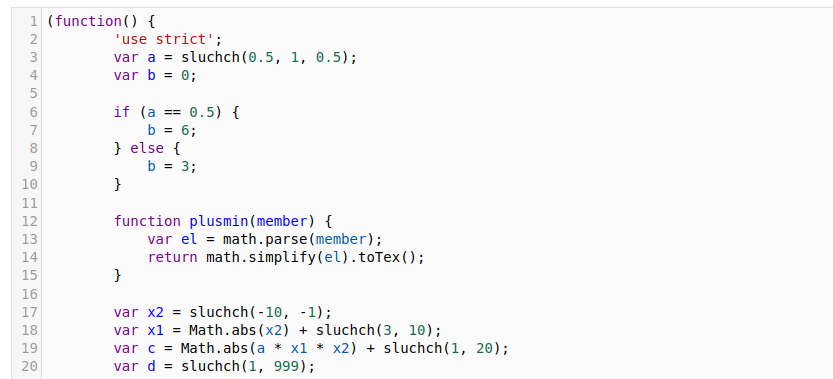
\includegraphics[width=1\linewidth]{VM/1.1.png}
	\end{figure}

Здесь объявляются переменные таким образом, чтобы генерируемые значения,  максимально соотносились с исходной задачей.

В этой части также используются специальные встроенные функции, такие как:
\\ \texttt{sluchch(a, b)} – функция случайным образом возвращает число из диапазона от «a» до «b». Если функции добавить третье число \texttt{sluchch(a, b, с)}, то она будет возвращать случайно число уже с шагом «с».
\\ \texttt{Math.abs(a)} – функция возвращает модуль числа «a».
\\ \texttt{function plusmin(member)} – функция принимает аргумент, содержащий в себе пример, наподобие: «1*a+-b». И возвращает его упрощённый вариант: «a-b».

Вторая часть выглядит следующим образом:

	\begin{figure}[h]
		\centering
		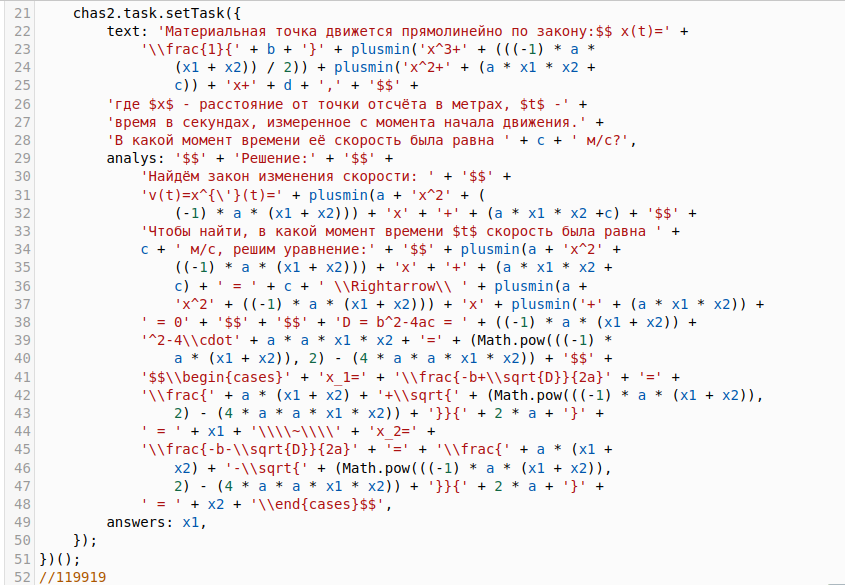
\includegraphics[width=0.8\linewidth]{VM/2.2.png}
	\end{figure}

Вторая часть программы делится на несколько составных частей:
\\ условие задачи, записанное после \texttt{text:}
\\ решение, записанное после \texttt{analys:}
\\ ответ, записанный после \texttt{answer}

В этом шаблоне мы вводим переменные, генерирующие случайные значения, которые используем для составления ответа. И на основе ответа мы уже составляем саму задачу и её решение.

В этой части также используются некоторый команды latex, например:
\\ \texttt{\textbackslash frac} – функция выводящая дробь на экран.
\\ \texttt{\textbackslash Rightarrow} – функция выводящая двойную стрелку вправо
\\ \texttt{\textbackslash begin\{cases\}} и \texttt{\textbackslash end\{cases\}} – окружение, выводящая фигурную скобку на экран.

\textbf{ Пример сгенерированных шаблоном задач}

 	\begin{figure}[h]
		\centering
		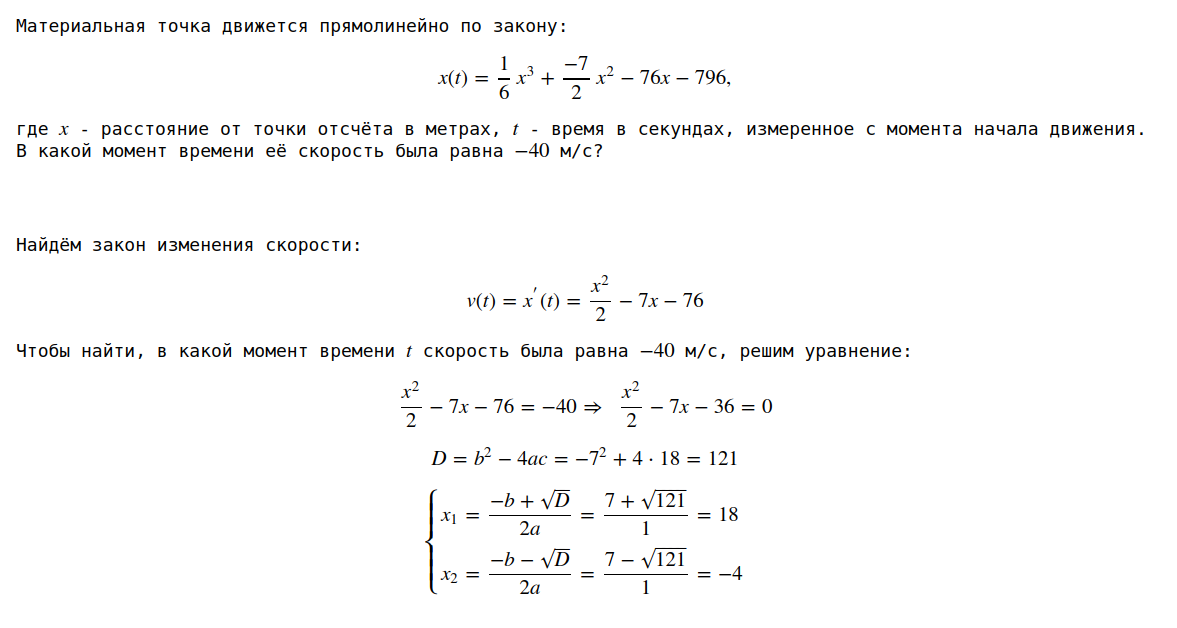
\includegraphics[width=0.85\linewidth]{VM/vch1.png}
		 		\end{figure}
		 	\begin{figure}[h]
		\centering
		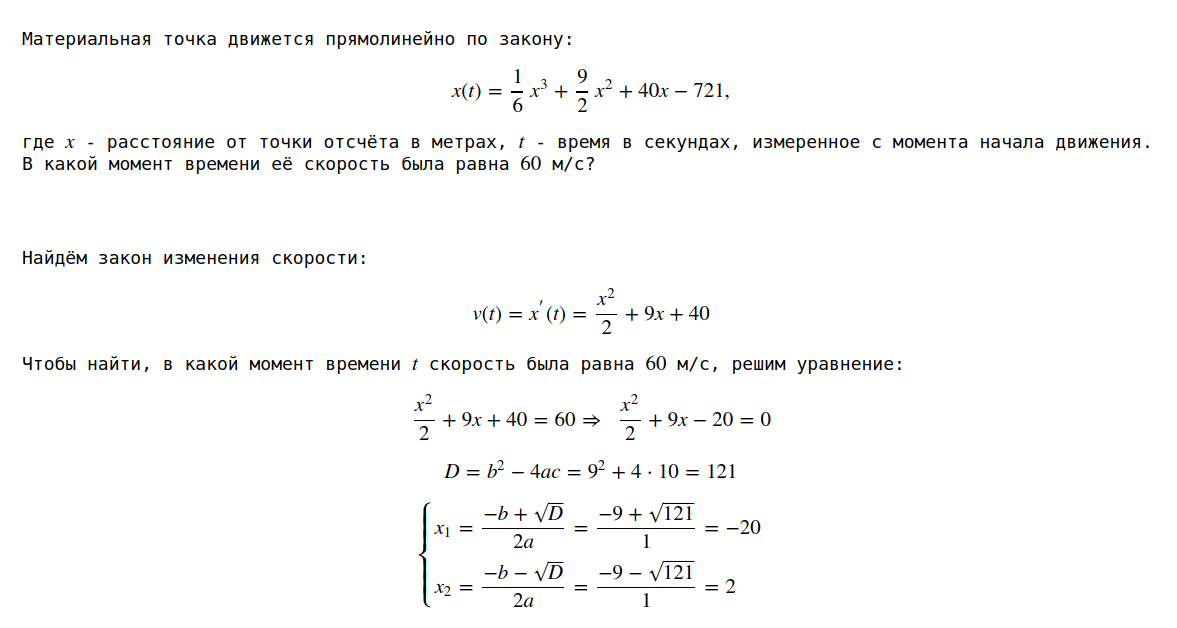
\includegraphics[width=0.85\linewidth]{VM/vch2.png}
	\end{figure}

\textbf{Задачи из ЕГЭ по математике базового уровня тип №16}
	\begin{figure}[h]
		\centering
		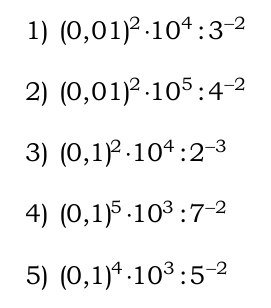
\includegraphics[width=0.25\linewidth]{VM/t16.1.png}
		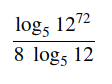
\includegraphics[width=0.15\linewidth]{VM/t16.3.png}
	\end{figure}
	
\textbf{Шаблоны задач}
\\
\begin{figure}[h]
		\centering
		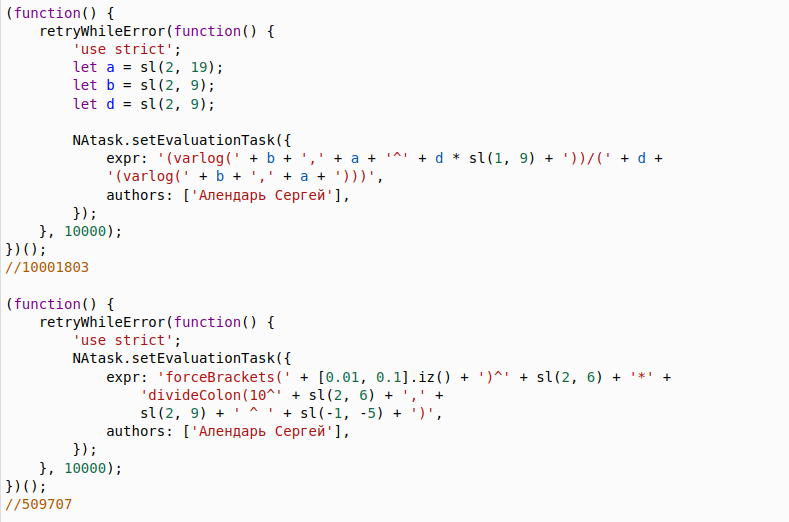
\includegraphics[width=0.8\linewidth]{VM/t16k.png}
	\end{figure}
	
Отличительной особенностью этих шаблонов от предыдущего, является другая библиотека - \texttt{setEvaluationTask}. Помимо самой генерации задачи, на основе переменных их первой части, она так же сама решает сгенерированный пример, и проверяет его ответ. 

Если ответ не является удовлетворительным, а именно таким, что пользователь просто не сможет ввести его на клавиатуре (Ответ представляет из себя бесконечную десятичную дробь, или просто очень длинную), то программа, отслеживает эту ошибку с помощью цикла \texttt{retryWhileError} и предпринимает ещё попытку составить задание с цельным ответом. Количество таких попыток указано внизу кода программы. Если за установленное число попыток, программа так и не получит правильно сгенерированную задачу, то она выведет сообщение об ошибке.

В этих шаблонах тоже используются некотрые свои специальные встроенные функции, например:
\\ \texttt{varlog} - отвечает за отображение логарифма на экране.

Также эта библиотека способна сама убирать некоторые скобки, если они не влияют на решение задания, или сама выполнть арифметическую операцию. Но в некотрых случаях, это не является необходимостью. Чтобы программа не высчитывала сама, то что стоит оставить, используются следующие команды:
\\ \texttt{forceBrackets} - для сохранение скобок.
\\ \texttt{divideColon} - для вывода знака деления «:».

\textbf{Сгенерированные по шаблонам задания}

\begin{figure}[h]
		\centering
		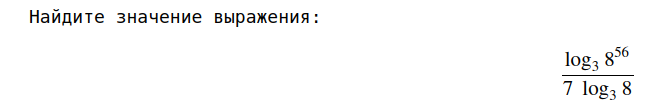
\includegraphics[width=0.6\linewidth]{VM/log1.png}
		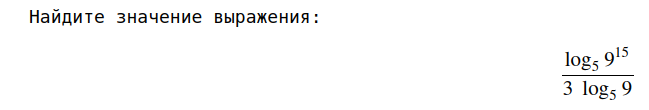
\includegraphics[width=0.6\linewidth]{VM/log2.png}
		\end{figure}
		\begin{figure}[h]
		\centering
		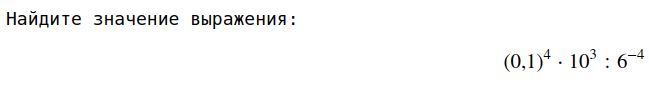
\includegraphics[width=0.6\linewidth]{VM/skob1.png}
		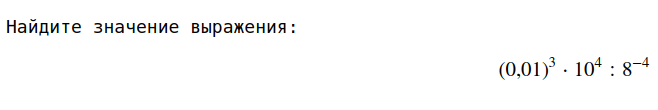
\includegraphics[width=0.6\linewidth]{VM/skob2.png}
\end{figure}

\textbf{Задача №77381 тип №6}

\begin{figure}[h]
	\centering
	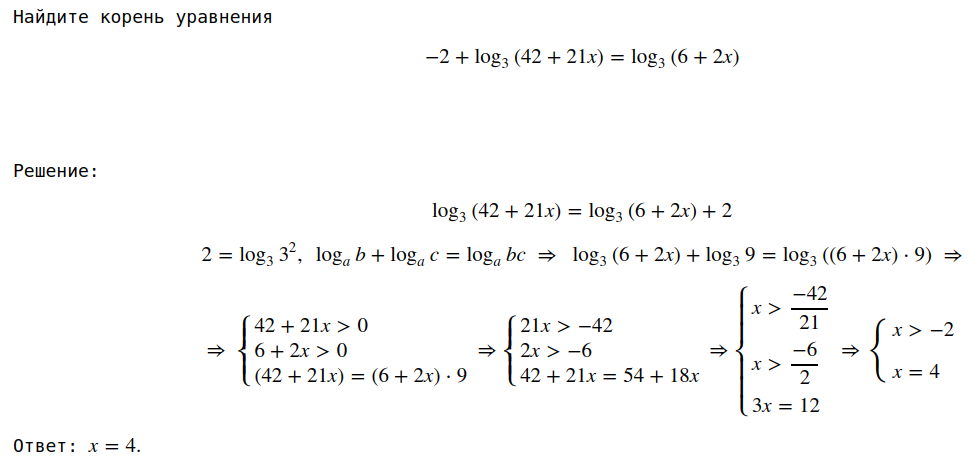
\includegraphics[width=0.9\linewidth]{VM/log.png}
\end{figure}

\newpage

Первая часть шаблона
	
\begin{figure}[h]
		\centering
		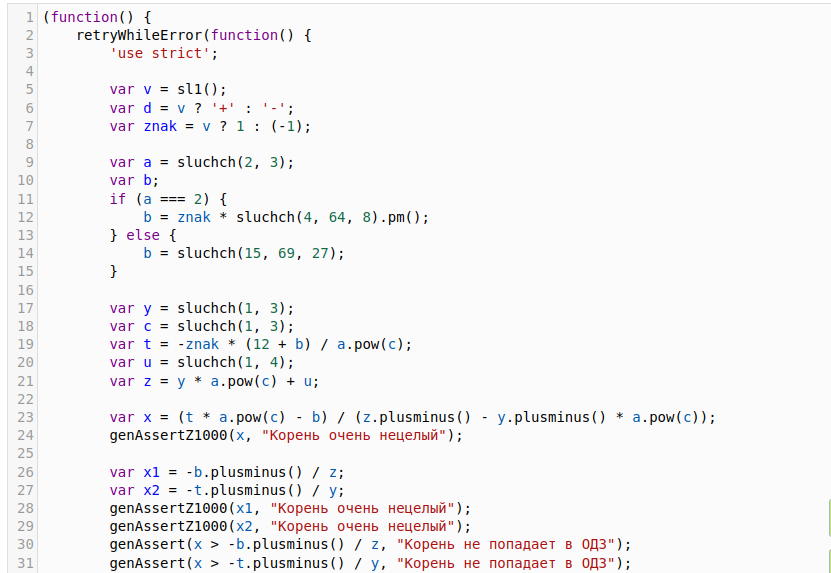
\includegraphics[width=0.9\linewidth]{VM/1log.png}
		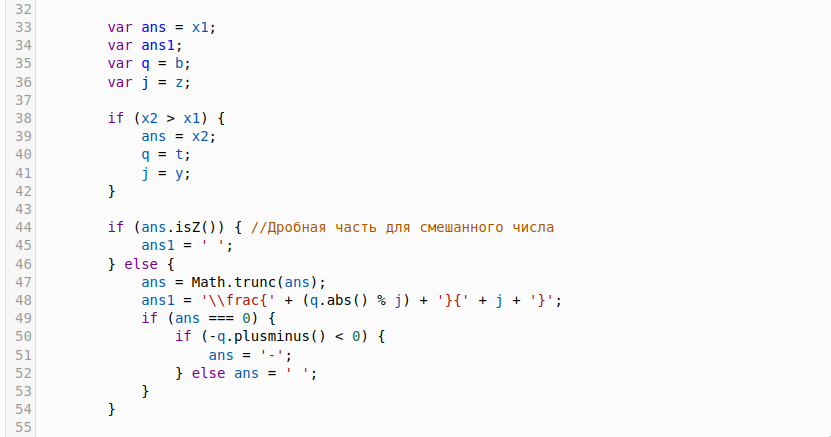
\includegraphics[width=0.9\linewidth]{VM/2log.png}
\end{figure}

\newpage

Вторая часть шаблона

\begin{figure}[h]
		\centering
		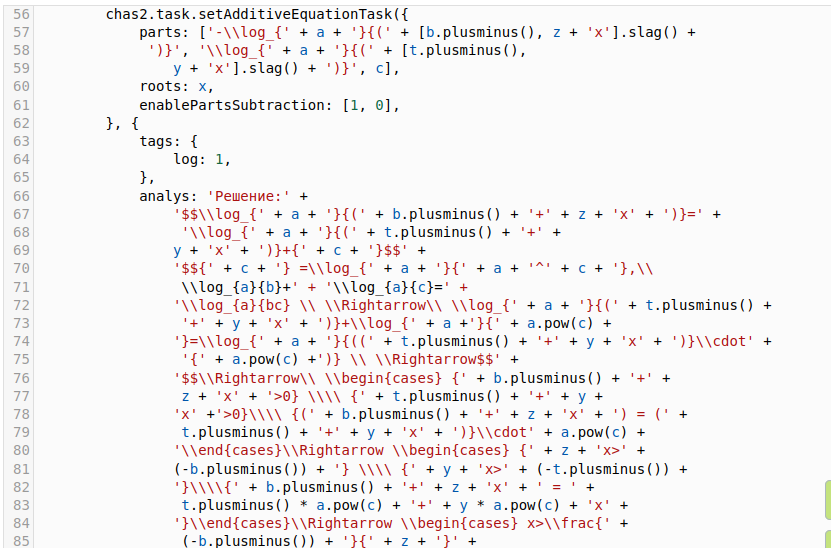
\includegraphics[width=0.96\linewidth]{VM/3log.png}
		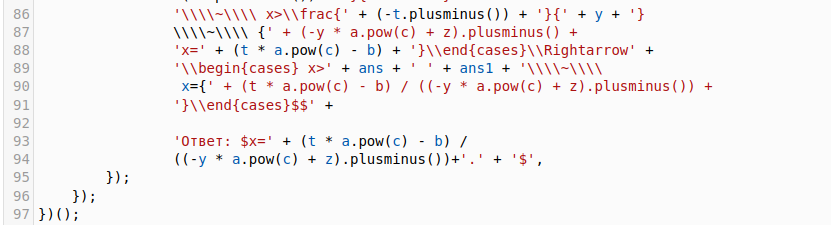
\includegraphics[width=0.96\linewidth]{VM/4log.png}
\end{figure}

\textbf{Задачи, сгенерированные по шаблонам, использующим код арифметической прогрессии.}
	\begin{figure}[h]
		\centering
		
\includegraphics[width=1\linewidth]{VM/1 (1).png}
		
\includegraphics[width=1\linewidth]{VM/2 (1).png}
		
\includegraphics[width=1\linewidth]{VM/3 (1).png}
	\end{figure}
	
\newpage

\textbf{Код арифметической прогрессии}

	\begin{figure}[h]
		\centering
		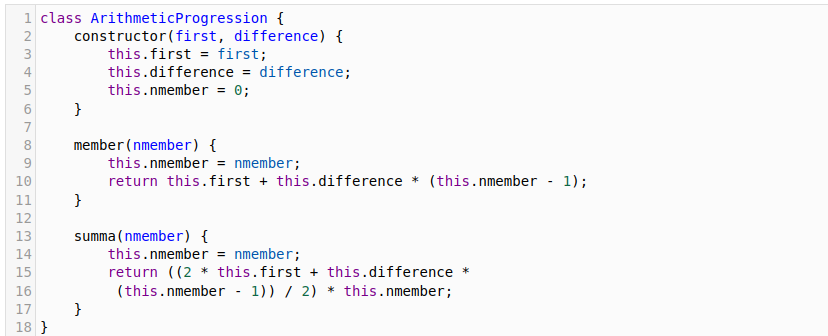
\includegraphics[width=1.1\linewidth]{VM/3b.png}
		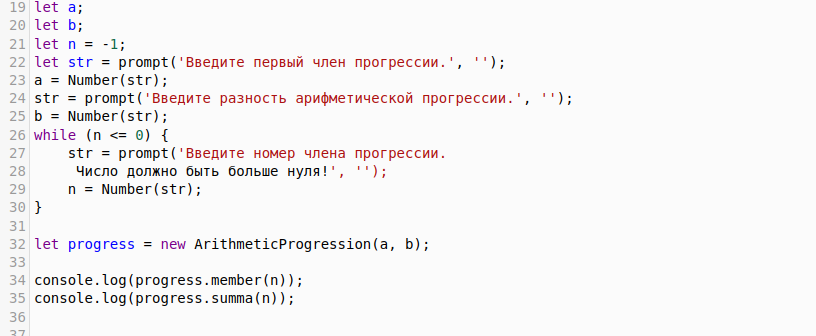
\includegraphics[width=1.1\linewidth]{VM/3c.png}
	\end{figure}

\textbf{Задачи, сгенерированные по шаблонам, использующим код 
\\геометрической прогрессии.}

	\begin{figure}[h]
		\centering
		
\includegraphics[width=1\linewidth]{VM/4 (1).png}
		
\includegraphics[width=1\linewidth]{VM/5 (1).png}
	\end{figure}
	
\textbf{Код геометрической прогрессии}

\newpage

\begin{figure}[h]
		\centering
		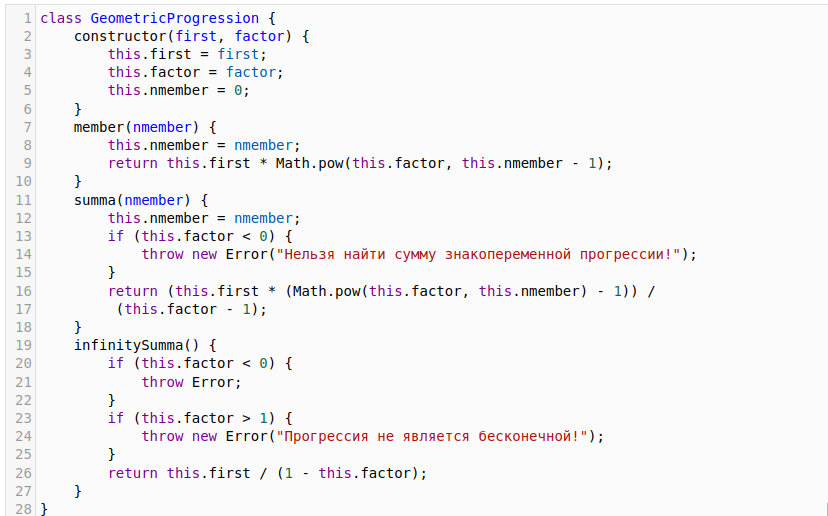
\includegraphics[width=0.9\linewidth]{VM/4b.png}
		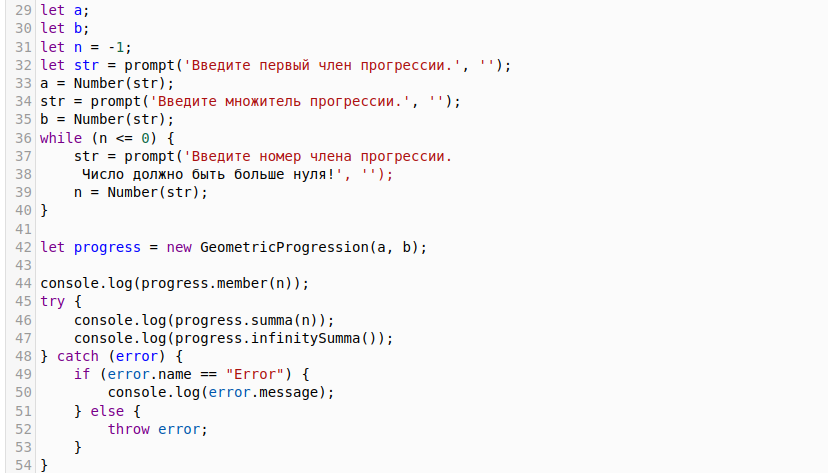
\includegraphics[width=0.9\linewidth]{VM/4c.png}
	\end{figure}
	
\newpage

\textbf{Тригонометрическая задача №77492}

	\begin{figure}[h]
		\centering
		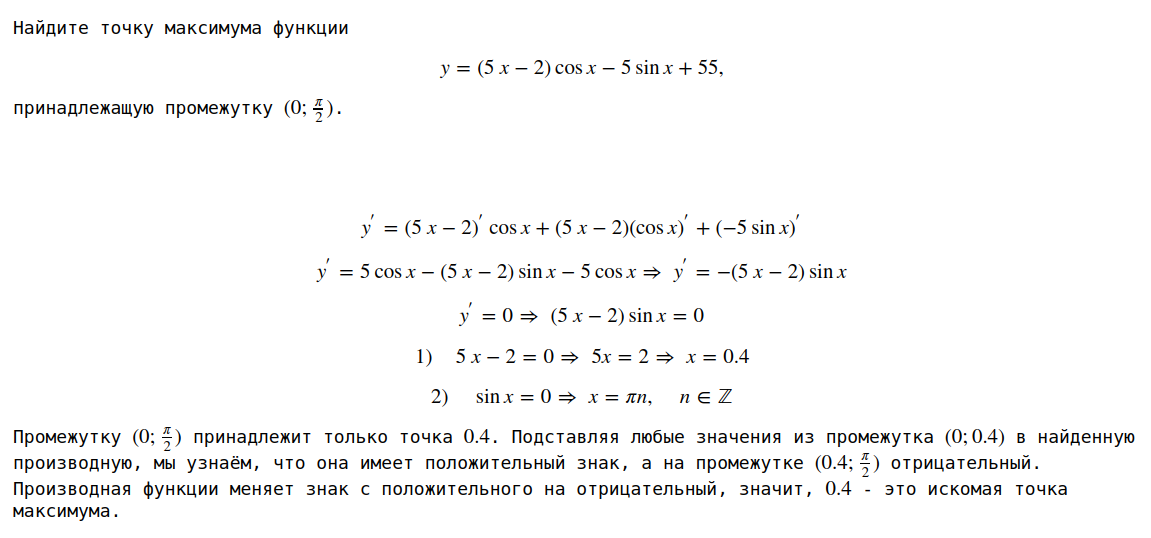
\includegraphics[width=1\linewidth]{VM/7 (1).png}
	\end{figure}

\textbf{Код для задачи №77492}

\begin{figure}[h]
		\centering
		\includegraphics[width=1\linewidth]{VM/7б.png}
\end{figure}
			
\begin{figure}[h]
		\centering
		\includegraphics[width=1\linewidth]{VM/7в.png}
\end{figure}
\newpage


\section*{Заключение}
\addcontentsline{toc}{section}{Заключение}
За всё время работы было разработано следующее количество шаблонов:
\\Тип №10 ЕГЭ профильного уровня на арифметические прогрессии: \textbf{9}
\\Тип №10 ЕГЭ профильного уровня на геометрические прогрессии: \textbf{2}
\\Тип №6 ЕГЭ профильного уровня на логаифмические уравнение: \textbf{3}
\\Тип №8 ЕГЭ профильного уровня на физический смысл производной,
\\ нахождение скорости процесса: \textbf{1}
\\Тип №12 ЕГЭ профильного уровня на наибольше и наименьшее 
\\значение функции: \textbf{12}
\\Тип №16 ЕГЭ базового уровня на вычисления и преобразования: \textbf{23}

Также были подготовлены тезисы, которые были отправлены для заочного участия в 74 МСНТК.

Данная работа помогла оказать вклад в развитии образовательного проекта «Час ЕГЭ», а разработанные шаблоны, будут способствовать в подготовке школьников к тестовой части ЕГЭ по математике. 

Помимо этого, сама дипломная работа будет служить руководством для будущих студентов, которые будут также принимать участие в разработке шаблонов и развитии проекта "Час ЕГЭ".





\newpage

\section*{Список использованных источников}
\setlength{\parindent}{0cm}
\addcontentsline{toc}{section}{Список использованных источников}
\addcontentsline{toc}{chapter}{Литература}
\begin{thebibliography}{99}

\bibitem{VirtualBox}VirtualBox. Виртуальные диски. Их типы. Расширение виртуального носителя // Хекслет Рус : [сайт]. - 2021. - URL: https://ru.hexlet.io/blog/posts/virtualbox-virtualnye-diski-ih-tipy-rasshirenie-virtualnogo-nositelya (Дата обращения 22.03.2024)

\end{thebibliography}

1.\quad VirtualBox. Виртуальные диски. Их типы. Расширение виртуального носителя // Хекслет Рус : [сайт]. - 2021. - URL: https://ru.hexlet.io/blog/posts/virtualbox-virtualnye-diski-ih-tipy-rasshirenie-virtualnogo-nositelya (Дата обращения 22.03.2024)
\\ 2. \quad Колесников Е. Н. Что такое GitHub и как им пользоваться / Е. Н. Колесников // SkillBox Media : [сайт]. - 2024. - URL:https://skillbox.ru/media/code/chto-takoe-github-i-kak-im-polzovatsya/ (Дата обращения: 02.04.2024)
\\3.\quad \textbf{Львовский С. М.} «Набор и верстка в системе LaTeX» - URL: https://old.mccme.ru//free-books//llang/newllang.pdf (дата обращения: 16.04.2024).
\\4.\quad Образовательный портал «РЕШУ ЕГЭ» - URL: https://ege.sdamgia.ru 
\\5.\quad Открытый банк задач ЕГЭ по Математике. Профильный уровень. – URL: https://prof.mathege.ru
\\6.\quad Полноценная платформа для разработчиков для создания, масштабирования и доставки защищенного программного обеспечения GitHub — URL: https://github.com/nickkolok/chas-ege/ (дата обращения: 20.04.2024).  
\\7.\quad Полный интерактивный тест - Тренажёр «Час ЕГЭ» - URL:https://math.vsu.ru/chas-ege/sh/polnmat.html (дата обращения: 18.04.2024).
\newpage

\appendix

\end{document}